\subsection{Facial Detection and Recognition}

Since simple image operations mentioned earlier can be done within a homomorphic cryptosystem, these operations can be assembled together in order to do more complex operations. A prominent application of image processing that often uses complex image operations is \textit{facial recognition}.

Traditional facial recognition algorithms rely on detecting salient features in a face image. Proposed by Matthew Turk and Alex Pentland, the \textit{eigenfaces} method uses principal component analysis (PCA) in order to express an input image as a linear combination of eigenfaces \cite{turk_eigenfaces_1991}. An \textit{eigenface} is a principal component, or more simply an eigenvector that represents a certain variation between the face images which are taken from the initial training set. The number of resulting eigenfaces is equal to the number of face images in the training set.
% One of the popular facial recognition algorithms is \textit{eigenfaces}.
% Traditional facial recognition algorithms rely on detecting salient features in a face image. Two of the popular facial recognition algorithms are \textit{eigenfaces} and \textit{Haar cascades}.

% \subsubsection{Eigenfaces}


% In the enrollment process, $M$ face images $\Theta_1, \ldots, \Theta_M$, each of size $p \times q$, are taken in to comprise the initial training set. The training images can be represented as vectors of length $N = pq$, where each row of an image is concatenated together.

% The average of the training images, denoted as $\Psi$, is
% \begin{equation}
% 	\Psi = \frac{1}{M} \sum_{i=1}^{M} \Theta_i
% \end{equation}

% The \textit{difference vectors} are then computed as $\Phi_i = \Theta_i - \Psi$. PCA is applied on the covariance matrix of the vectors
% \begin{equation}
% 	\mathbf{C} = \frac{1}{M} \sum_{i=1}^M \Phi_i \Phi_i^\top = \frac{1}{M} \mathbf{A}\mathbf{A}^\top,
% \end{equation}
% where $\mathbf{A}$ is an $N \times M$ matrix defined by $\left[\Theta_1 \quad \Theta_2 \quad \cdots \quad \Theta_M\right]$, in order to determine the orthonormal eigenvectors \cite{hutchison_privacy-preserving_2009}.

% Directly computing the covariance matrix and then applying PCA will become inefficient for large sizes of $\mathbf{A}$, since computing for $\mathbf{A}\mathbf{A}^\top$ results in an $N \times N$ matrix, which can get drastically large because it is dependent on the size of the image. On the other hand, computing for $\mathbf{A}^\top\mathbf{A}$ only results in an $M \times M$ matrix, which is much smaller than the previous one because it is just dependent on the number of face images in the training set. Now, we can apply PCA to $\mathbf{A}^\top\mathbf{A}$ along with some post-processing to obtain the eigenvectors \cite{hutchison_privacy-preserving_2009}.

% Instead of getting the eigendecomposition of the covariance matrix by explicitly computing the eigenvalues and eigenvectors of $\mathbf{C}$, we can also apply \textit{singular value decomposition} (SVD) on the matrix $\Phi^\top$. This is because SVD works through a divide-and-conquer method which results in greater numerical stability, while eigendecomposition simply uses the traditional QR factorization \cite{nakatsukasa_stable_2013, gu_divide-and-conquer_1995}. Upon applying SVD, we now get the eigenvectors $\mathbf{u}_1, \ldots, \mathbf{u}_M$ and their corresponding eigenvalues $\lambda_1, \ldots, \lambda_M$.

% We choose $K$ eigenvectors $\mathbf{u}_1, \ldots, \mathbf{u}_K$ such that it comprises a set associated with the $K$ largest eigenvalues, where $K$ is much smaller than $M$. This set is now the \textit{face space}. Then, the images $\Theta_1, \ldots, \Theta_K$ are projected onto the face space spanned by the eigenfaces to determine the weight vectors $\Omega_1, \ldots, \Omega_K$.

% To perform the recognition process, the algorithm projects the input image $\Gamma$ onto the face space, and then comparing the projected image $\bar{\Omega} = \mathbf{u}_i\left(\Gamma - \Psi\right)$ with each eigenface in the face space using a metric such as the Euclidean distance. Thus it is computed as $d_i = \left\lVert \Omega_i -\bar{\Omega} \right\rVert$ for all $i=1,\ldots,K$, where $\left\lVert \cdot \right\rVert$ denotes the Euclidean norm.

% Then, a match can be reported if the smallest possible distance is smaller than the given threshold value $T$.
% \newcommand{\argmin}{\mathop{\mathrm{arg\,min}}}
% \begin{equation}
% 	\text{ID} = \begin{cases}\argmin_i d_i & \text{if } \min_i d_i \le T \\\emptyset & \text {otherwise}\end{cases}
% \end{equation}


% \subsection{Previous Implementations of Secure Facial Recognition}
Erkin, et al. \cite{hutchison_privacy-preserving_2009} devised a method to incorporate the use of homomorphic cryptosystems into the eigenfaces method, primarily using the Paillier cryptosystem. In their study, they proposed a two-party system where Alice holds an encrypted image $\left[\Gamma\right]$, while Bob maintains a database of $K$ eigenfaces $\mathbf{u}_1, \ldots, \mathbf{u}_K$, and feature vectors $\Omega_1, \ldots, \Omega_M$ in the plaintext domain.

\begin{figure}[h]
    \centering
    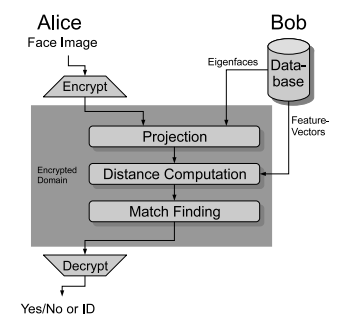
\includegraphics[width=0.4\textwidth]{figures/secure_eigenfaces.png}
    \caption{Diagram of the privacy-preserving facial recognition process, from \cite{hutchison_privacy-preserving_2009}}
\end{figure}

In order to ensure privacy, the steps in the eigenfaces algorithm, namely: projection, distance computation, and match finding, are done within the encrypted domain, i.e., using the operations in the Paillier cryptosystem.

Projection is similar to that of the original eigenfaces algorithm, except the operations are replaced with their respective operations in the cryptosystem. Distance computation in this version is somewhat different from the original eigenfaces method, in that it deals with the square of the Euclidean distance since the relative order of the distances is only important when comparing these during the match finding step \cite{hutchison_privacy-preserving_2009}.
\begin{align}
    d_i &= \left\lVert \Omega_i - \bar{\Omega} \right\rVert ^2 = \sum_{j=1}^{K} \left(\omega_{ij} - \bar{\omega}_j\right)^2 \\
        &= \underbrace{\sum_{j=1}^{K} \omega_{ij}^2}_{\mathcal{S}_1} + \underbrace{\sum_{j=1}^{K} \left(-2 \omega_{ij} \bar{\omega_j}\right)}_{\mathcal{S}_2} + \underbrace{\sum_{j=1}^{K} \bar{\omega}_{j}^2}_{\mathcal{S}_3}
\end{align}

Computing for the distances within Paillier would just be multiplying the encrypted sums together.
\begin{equation}
	\left[d_i\right] = \left[\mathcal{S}_1\right] \cdot \left[\mathcal{S}_2\right] \cdot \left[\mathcal{S}_3\right]
\end{equation}
The terms $\left[\mathcal{S}_1\right]$ and $\left[\mathcal{S}_2\right]$ can be easily computed by Bob, since he already knows both $\omega_i$ in the clear and $\left[\bar{\omega}_i\right]$ which is in encrypted form. Computing for $\left[\mathcal{S}_3\right]$ requires the use of the secure squaring protocol outlined in Table \ref{tab:flop_summary}.
% The terms $\left[\mathcal{S}_1\right]$ and $\left[\mathcal{S}_2\right]$ can be easily computed by Bob, since he already knows both $\omega_i$ in the clear and $\left[\bar{\omega}_i\right]$ which is in encrypted form. Computing for $\left[\mathcal{S}_3\right]$ is trickier because Bob cannot compute for $\left[\bar{\omega}_i^2\right]$ because pairwise multiplication is not supported in Paillier, that is why Bob needs help from Alice to square a number through a protocol described below \cite{hutchison_privacy-preserving_2009}.

% Before Bob sends $\left[\bar{\omega}_i\right]$ to Alice for squaring, he adds a random number $r_i$ to compute $\left[x_i\right] = \left[\bar{\omega}_i + r_i\right] = \left[\bar{\omega}_i\right] \cdot \left[r_i\right]$, where $r_i$ is obviously distinct for every $i$, then sends $\left[x_i\right]$ to Alice. She then decrypts it and computes $x_i^2$, and then computes $\mathcal{S}_3^\prime = \sum_{i=1}^{K} x_i^2$, after which she encrypts the sum and sends $\left[\mathcal{S}_3^\prime\right]$ to Bob. Now, he can compute for $\left[\mathcal{S}_3\right]$ as follows:
% \begin{equation}
% 	\left[\mathcal{S}_3\right] = \left[\mathcal{S}_3^\prime\right] \cdot \prod_{j=1}^{K} \left(\left[\bar{\omega}_j\right]^{-2r_j} \cdot \left[-r_j^2\right]\right)
% \end{equation}

% The protocol for squaring a number as described earlier is a workaround for the limitations of Paillier or any other partially homomorphic cryptosystem that only supports addition and scalar multiplication.
% This can be possibly extended so that operations such as pairwise multiplication and exponentiation are also supported, provided that the protocol involves two parties.

The match-finding step is done by comparing the distances obtained from the previous step to a specified threshold $T$. If the minimum distance is smaller than $T$, then a match is found, and the encrypted identity of the match is returned to Alice \cite{hutchison_privacy-preserving_2009}. Getting the minimum among the encrypted distances involves comparing two numbers which can be performed using the DGK secure comparison protocol \cite{pieprzyk_efficient_2007}.
